\section{Data notes}
\subsection{Putting density in perspective}
\paragraph{Spacial distribution} where are the densest CZ? See panel a of Figure \ref{fig:map}
\begin{figure}[!h]
\centering
\caption{The geography of population density and its persistence}
\subfloat[Population density in 2010]{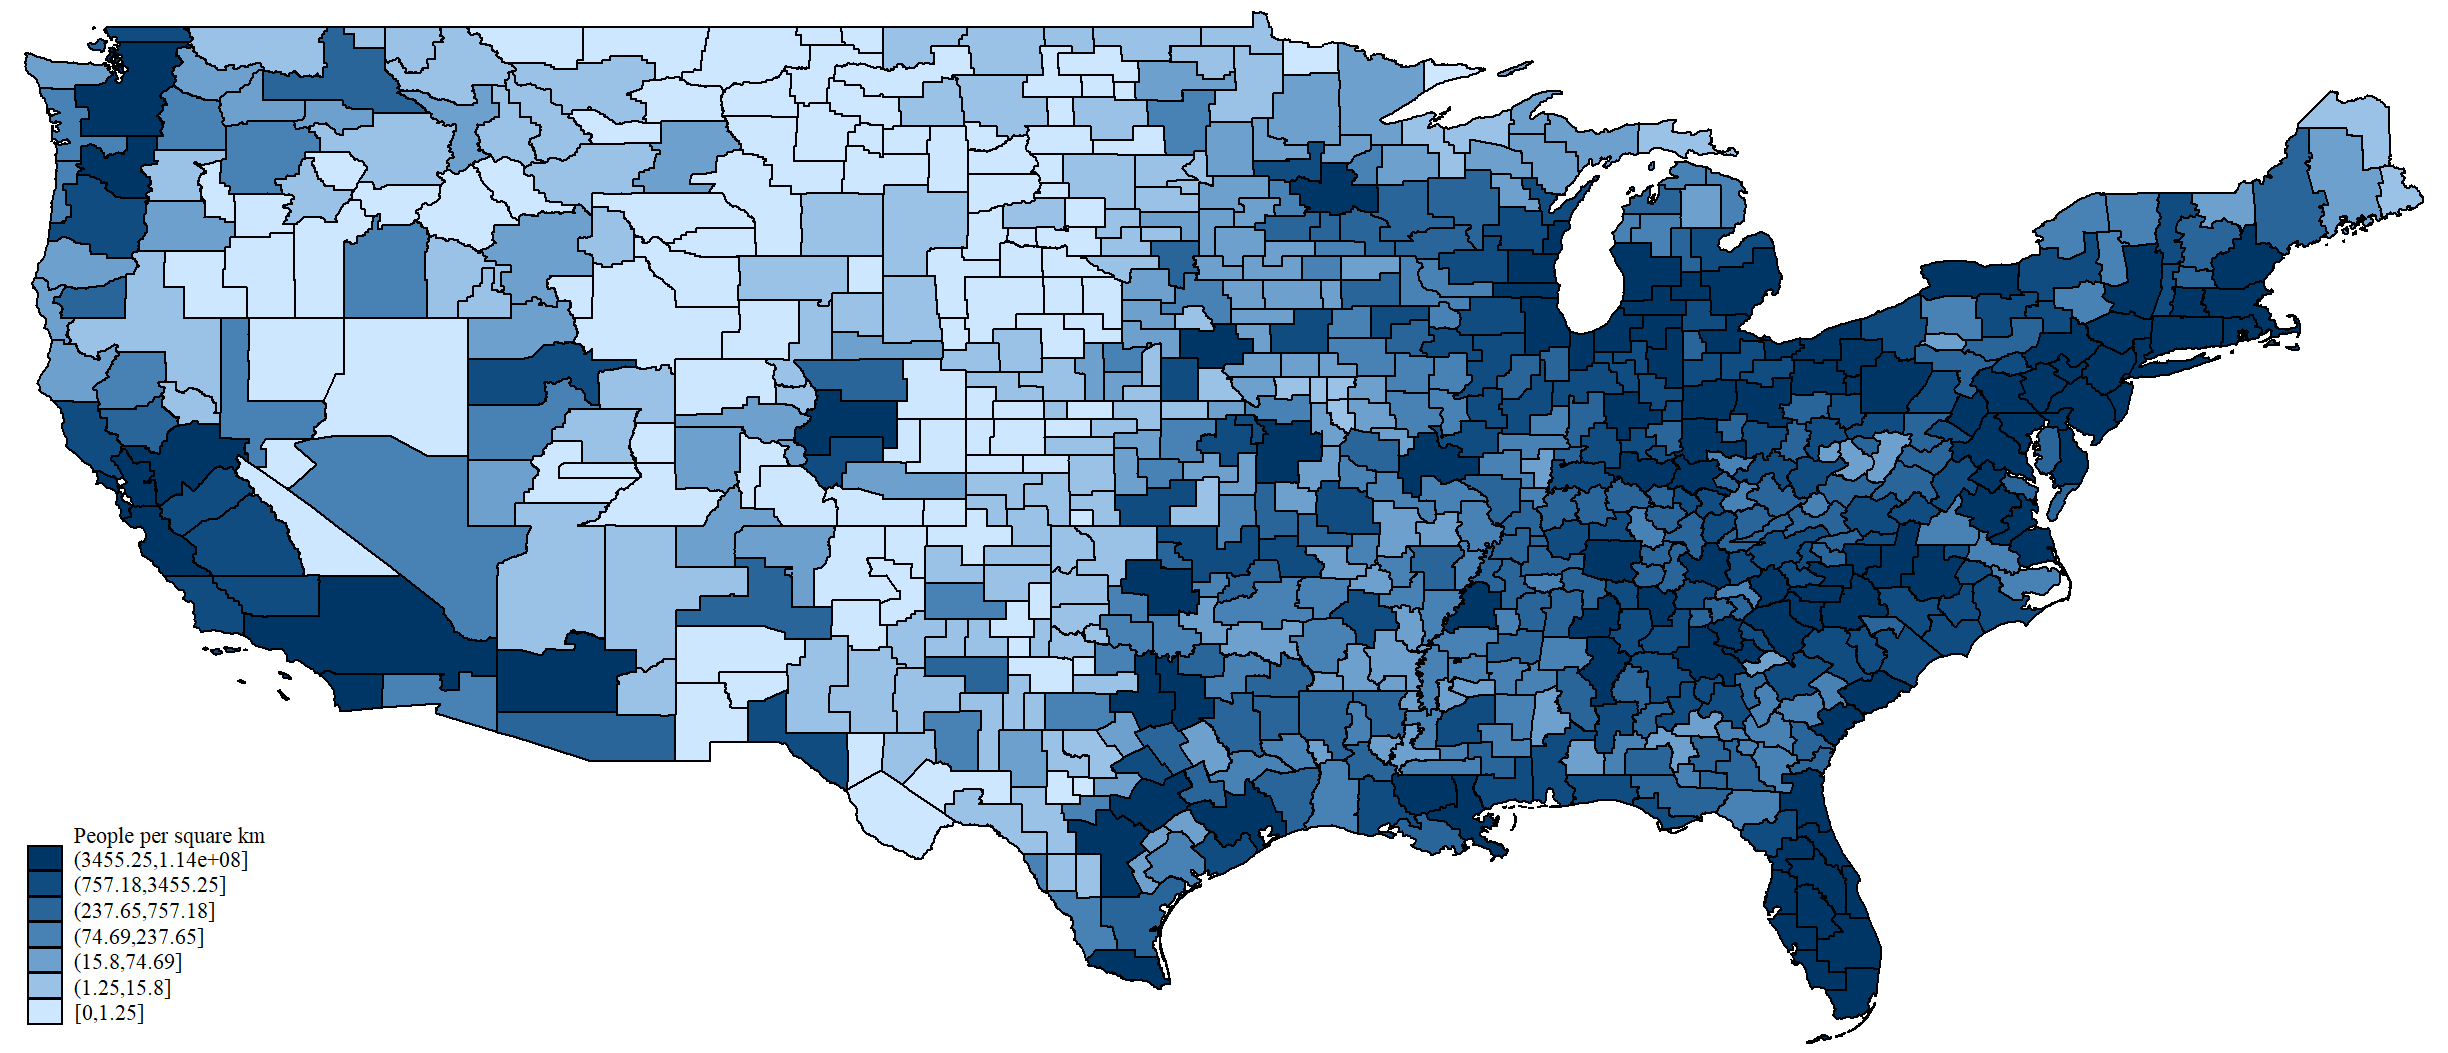
\includegraphics[width=1\textwidth]{../2_analysis/output/figures/czone_density2010}} \\ \subfloat[Density in 2010 vs 1950]{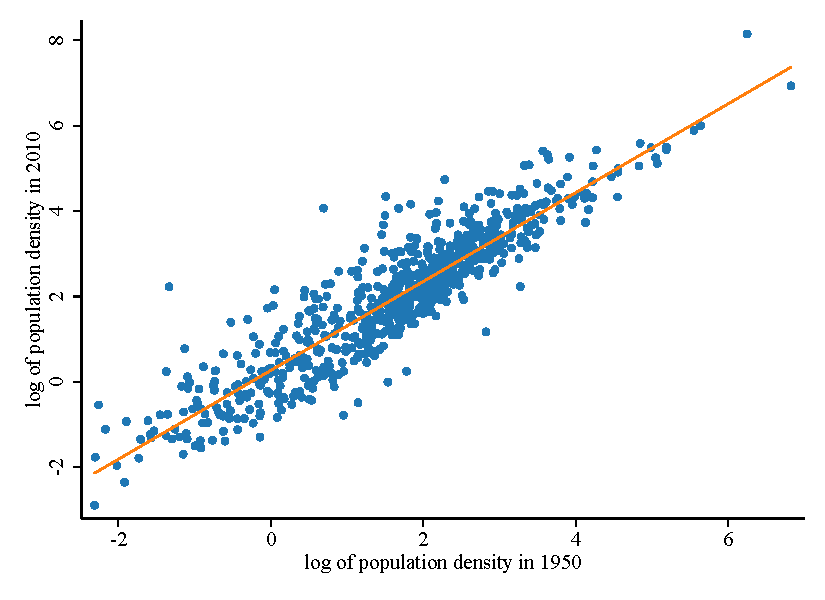
\includegraphics[width=1\textwidth]{../2_analysis/output/figures/persistence_population_density}} \\ 
\par \begin{minipage}[h]{\textwidth}{\scriptsize\textbf{Note:} Figure restricts to czones with population densities above 1 person per km$^2$ and full-time year-round workers..}\end{minipage}
\end{figure}



\paragraph{Persistence:} panel b of figure \ref{fig:map} shows that density is highly persistent. The slope coefficient from the regression in the figure is 1.04.

\paragraph{Summary statistics} selected summary statistics for the 625 CZ in my sample are shown in table \ref{tab:summary_statistics}.


\begin{table}
\caption{Selected summary statics for CZ, 2020}
\label{tab:summary_statistics}
\begin{tabular}{l*{1}{cccccc}} \hline\hline
                    &\multicolumn{6}{c}{}                                                         \\
                    &       count&         p10&         p25&         p50&         p75&         p90\\
\hline
log of population density&         625&    .6182053&    1.489836&    2.357417&    3.144841&    4.051244\\
wage\_raw\_gap        &         625&    .1288653&    .1587546&    .1871793&    .2173289&    .2517551\\
\hline\hline
\end{tabular}

\end{table}

\paragraph{What are the densest CZ?}
Table \ref{tab:cz_examples} shows examples of CZ at different points of the density distribution. Whenever available, the table lists the main city in the CZ.
\begin{table}[tbp] \centering
\newcolumntype{C}{>{\centering\arraybackslash}X}

\caption{Examples of CZ at different percentiles of population density in 2020}
\label{tab:cz_examples}
\begin{tabularx}{\textwidth}{lCCCCC}

\toprule
&{(1)}&{(2)}&{(3)}&{(4)}&{(5)} \tabularnewline
{Percentile}&{Main city}&{State}&{log of population density}&{Population density}&{Total population} \tabularnewline
\midrule\addlinespace[1.5ex]
1&undefined&Texas&-.43&.65&7577 \tabularnewline
1&undefined&South Dakota&-.49&.61&1424 \tabularnewline
5&undefined&Texas&.16&1.18&4933 \tabularnewline
5&undefined&South Dakota&.14&1.16&10137 \tabularnewline
10&undefined&Kansas&.62&1.86&16528 \tabularnewline
10&undefined&Nebraska&.61&1.84&5473 \tabularnewline
25&undefined&Wyoming&1.49&4.44&55507 \tabularnewline
25&undefined&California&1.49&4.43&78207 \tabularnewline
50&undefined&Missouri&2.36&10.56&84805 \tabularnewline
50&undefined&Illinois&2.36&10.56&72896 \tabularnewline
75&undefined&West Virginia&3.14&23.22&180731 \tabularnewline
75&undefined&Pennsylvania&3.14&23.14&198774 \tabularnewline
90&undefined&North Carolina&4.05&57.47&253676 \tabularnewline
90&Youngstown OH&Ohio&4.03&56.53&386753 \tabularnewline
95&Fort Worth TX&Texas&4.46&86.08&1340106 \tabularnewline
95&Reading PA&Pennsylvania&4.43&84.09&652241 \tabularnewline
99&Baltimore MD&Maryland&5.49&241.41&1476239 \tabularnewline
99&Philadelphia PA&Pennsylvania&5.44&229.79&3178354 \tabularnewline
100&Miami FL&Florida&8.15&3462.06&2550814 \tabularnewline
100&New York City NY&New York&6.93&1027.16&6829386 \tabularnewline
\bottomrule \addlinespace[1.5ex]

\end{tabularx}
\begin{flushleft}
\footnotesize \textbf{Note:} figure restricts to czones with population densities above 1 person per km$^2$
\end{flushleft}
\end{table}



\subsection{Residualization procedure}
Throughout this document I explore the relationship between average wages (gender wage gap) and CZ population density. I am also interested in how this relationship has changed over time.

To discard the possibility that the observed relationships arise because of simple changes in the population composition, I compute average wages net of individuals' characteristics.

\paragraph{Procedure}
\benu
	\item I regress log of the individuals' wages on individual characteristics separately by year, including a gender $\times$ CZ fixed effect. Models are estimated separately for each census year.
	\beqns
		w_{igrt}=X_{irt}\gamma_t+\lambda_{rt}^g
	\eeqns
	\item $\hat{\lambda}_{grt}$ is my estimate of CZ wages, net of individual characteristics.
	\item I compute the CZ-specific gender gap as:
	\beqns
		gap_{rt}=\hat{\lambda}_{rt}^m-\hat{\lambda}_{rt}^f
	\eeqns
\eenu

Throughout the document, the control variables $X_{irt}$ come into for different sets:
\bitem
	\item \textbf{Basic controls:} age dummies, race dummies, and foreign born dummy.
	\item \textbf{Human capital:} basic controls + 4-level education dummies.
	\item \textbf{Industry controls:} human capital controls + $\approx$ 150 industry fixed effects.
	\item \textbf{Full controls:} industry controls + occupation fixed effects.
\eitem